%!TEX root = ../dokumentation.tex

\chapter{Evaluation}\label{cha:Evaluation}

\paragraph{Used example geometry and shaders}

For a basic example a scene consisting out of a tetrahedron which is rendered in three instances is chosen. These instances get different color and different transformations as shown in  \autoref{fig:exampleScene}.

The example for a vertex shader is applying the instance transformation to the vertex position and to its normal, applying a camera transformation to the resulting position and passing through the instance color.

The example for the fragment shader receives the position, the normal and the instance color and applies a light calculation based on a given directional light and the camera position.

\begin{figure}[h!]
  \centering 
  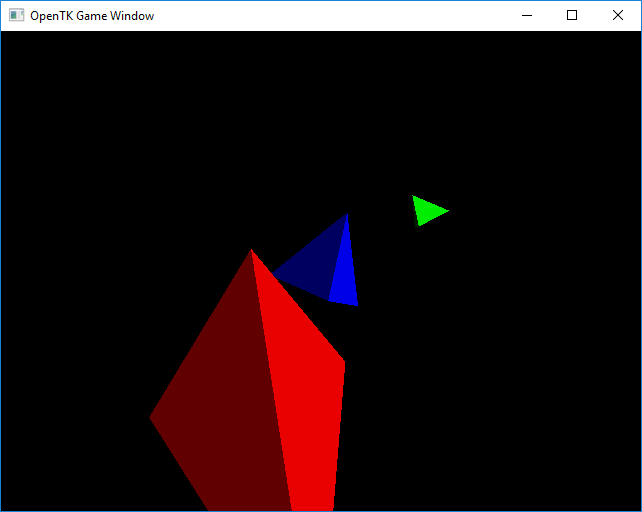
\includegraphics[scale=0.6]{scene.png}
  \caption[Screenshot of example scene of the project]{Project scene}
  \label{fig:exampleScene}
\end{figure}